\documentclass[a4paper,12pt]{report}
\usepackage[utf8]{inputenc}
\usepackage[T1]{fontenc}
\usepackage{lmodern}
\usepackage{eurosym}
\usepackage[french]{babel}
\usepackage{graphicx}

\usepackage{fancyvrb}
\usepackage{wrapfig}

\usepackage{hyperref}
\usepackage{float}


\setlength{\hoffset}{-18pt}
\setlength{\oddsidemargin}{0pt} % Marge gauche sur pages impaires
\setlength{\evensidemargin}{9pt} % Marge gauche sur pages paires
\setlength{\marginparwidth}{54pt} % Largeur de note dans la marge
\setlength{\textwidth}{461pt} % Largeur de la zone de texte (17cm)
\setlength{\voffset}{-18pt} % Bon pour DOS
\setlength{\marginparsep}{7pt} % Séparation de la marge
\setlength{\topmargin}{0pt} % Pas de marge en haut
\setlength{\headheight}{13pt} % Haut de page
\setlength{\headsep}{10pt} % Entre le haut de page et le texte
\setlength{\footskip}{27pt} % Bas de page + séparation
\setlength{\textheight}{708pt} % Hauteur de la zone de texte (25cm)

% Title Page
\title{Rapport de projet long \\ Attaques sur un AR Drone 2.0 Parrot}
\author{Kevyn \bsc{Ledieu}, Ferréol \bsc{Pennel}, Alexis \bsc{Pernot}}

\renewcommand{\thesection}{\arabic{section}}

\begin{document}
\maketitle
\tableofcontents
\newpage

\section{Introduction}
De plus en plus présents autour de nous, les drones de loisirs représentent à la fois des opportunités technologiques et des risques de sécurité. Régulièrement, nous pouvons observer des exemples de drones ayant perturber le trafic aérien par leur présence aux abords d'un aéroport. Ainsi un premier risque de sécurité qu'ils représentent est leur intégration dans l'espace aérien, espace que ces nouveaux aéronefs partagent avec de nombreux autres de toutes les tailles. Aussi des nouvelles règles sont à l'étude afin de réglementer ces activités de loisirs. Toutefois, même une fois réglementée et contrôlée, l'activité des drones de loisir présente un second risque de sécurité lié non plus à la gestion du drone par l'opérateur mais au drone lui-même. En effet, dans la course à l'innovation dans ce domaine porteur qu'est le drone de loisir, les entreprises négligent potentiellement l'aspect sécurité hardware et logicielle de leurs drones. Aussi, ceux-ci peuvent présenter de nombreuses vulnérabilités permettant à un attaquant extérieur de potentiellement prendre le contrôle du drone. Dans ce contexte, nous avons décidé d'étudier un drone grand public proposé par un des leaders du marché, la société \textit{Parrot}. Nous étudierons les différentes vulnérabilités potentiellement présentes sur ce drone et mettront en oeuvre un scénario d'attaque sous forme de tutoriel.

\section{Matériel et Méthode}
\subsection{Matériel: \bsc{AR Drone 2.0}}
Nous allons étudier un \bsc{AR Drone 2.0}. C'est un hélicoptère quadrirotor pilotable via une liaison WiFi au travers d'une application disponible sous iOS, Android, Linux ou Windows. C'est un drone civil principalement destiné au divertissement. Il est équipé de:
\medbreak
\begin{itemize}
    \item un \textit{processeur ARM Cortex A8 32 bits cadencé à 1 GHz}
    \item \textit{1 Go de RAM DDR2 cadencée à 200 MHz}
    \item un \textit{système d'exploitation Linux 2.6.32}
    \item un \textit{module WiFi b/g/n}
    \item un \textit{accéléromètre 3 axes}
    \item un \textit{gyroscope 3 axes}
    \item un \textit{capteur de pression}
    \item un \textit{un magnétomètre 3 axes}
    \item des \textit{capteurs de proximité à ultrasons}
    \item une \textit{caméra vericale QVGA}
    \item un \textit{port USB 2.0}
\end{itemize}

\newpage
\section{Hypothèse de travail}
Pour ce projet, nous supposerons que le drone utilisé est un ARDrone 2.0 qui n'a pas subi de modifications logicielles et qui est donc dans un état identique à sa sortie d'usine. Il dispose ainsi uniquement des protections éventuelles prévues par le constructeur Parrot. Nous supposons dans le cadre de ce projet que nous sommes  dans la position de l'attaquant et que l'ARDrone 2.0 est connecté et contrôlé par un client légitime.


\section{Présentation vulgarisée du travail}
\subsection{Premiers pas avec le drone}
Ce projet est centré sur la découverte de vulnérabilités sur l'ARDrone 2.0. Une première mise sous tension du drone nous a permis de découvrir que celui-ci propose un réseau Wifi ouvert, donc non protégé, permettant de se connecter à celui-ci et de le contrôler. Cette observation a grandement orienté notre travail. En effet, nous nous attendions à trouver un réseau Wifi sécurisé qu'il aurait été nécessaire de contourner ou de pénétrer afin d'avoir accès au drone. Cependant, le réseau ouvert nous permet en tant qu'attaquant de nous connecter directement au réseau Wifi créé par le drone. L'ARDrone 2.0 supporte la connexion de plusieurs clients simultanés à son réseau Wifi, toutefois seul le premier client a envoyer des paquets UDP de commande est maître du drone et a la possibilité de le contrôler. En supposant qu'un client légitime est connecté au drone, la question est: que peut faire l'attaquant ?

\subsection{Prise de contrôle du drone}
Une première idée est la prise de contrôle du drone par l'attaquant. Une fois connecté au réseau du drone, l'attaquant n'a qu'à déconnecter l'utilisateur légitime pour devenir le maître du drone. Ainsi en envoyant des messages au drone demandant la déconnexion du client légitime, l'attaquant est capable de prendre le contrôle du drone une fois celui-ci déconnecté.

\subsection{Injection de commandes}
Dans ce cas, le client légitime reste maître du drone. Toutefois l'attaquant se fait passer pour le client légitime et envoie des messages au drone. Il peut ainsi lui envoyer des instructions que le client légitime n'a jamais envoyé. Par exemple, l'attaquant peut envoyer au drone l'instruction d'atterrir à la place du client légitime.

\subsection{Virus sur le drone}
Ce troisième point exploite une faille importante du drone. En effet, celui-ci offre à tout utilisateur connecté à son réseau Wifi la possibilité d'accéder directement au système
d'exploitation du drone en ayant tous les droits sur celui-ci et sans authentification ni protection. Ainsi, en tant qu'attaquant connecté au réseau Wifi du drone, nous utilisons cet accès au drone pour déposer sur celui-ci un script. Celui-ci est chargé de copier une image sur toute clé USB connectée au drone afin de démontrer le potentiel de l'attaque. Il est en effet aisé de diffuser n'importe quel virus via clé USB grâce au drone et ceci sans difficultés particulières.

\subsection{Déni de service}
Cette attaque est une attaque de type "Homme du milieu". Dans cette situation, nous nous plaçons comme une passerelle entre le client et le drone, ce qui nous permet de contrôller tout le flux de communication entre les deux parties. Il est alors possible de bloquer le lien entre le drone et le client, ce qui créer donc une perte de liaison pour le client légitime

\subsection{Conclusion}
Ces quatre attaques différentes permettent de démontrer les vulnérabilités majeures que présente l'ARDrone 2.0. Une des failles principales de celui-ci est son réseau Wifi non protégé. La protection de celui-ci par du WPA2 permettrait de rendre ces quatre différentes attaques beaucoup plus complexes car l'attaquant aurait dans un premier temps besoin de casser le réseau Wifi. De plus, le drone offre des accès non protégés et privilégiés qui sont une faille majeure et permettent à un attaquant une prise de contrôle complète sur le drone.


\section{Présentation scientifique du travail}


\section{Tutoriel}
Le tutoriel du projet se présente sous la forme d'une application \textbf{Linux} développée en \textbf{Python} permettant d'exploiter les trois types d'attaques présentées précédemment. Disponible à l'adresse suivante: \url{https://github.com/ferreolpennel/Krokmou}, cette application de démonstration est utilisable par tout utilisateur satisfaisant les pré-requis à son installation. L'application, appelée \bsc{Krokmou}, est dédiée à l'ARDrone 2.0 et ne permet des attaques que contre ce type de drone et ce à des fins de démonstration uniquement. Elle permet ainsi de prendre le contrôle d'un drone à la place d'un utilisateur légitime déjà connecté au drone, d'envoyer des commandes pirates au drone sans déconnecter l'utilisateur légitime de celui-ci et de déposer un virus de démonstration sur le drone. Elle illustre ainsi les attaques présentées précédemment et met en relief les failles correspondantes sur ce type de drone.

\subsection{Initialisation de l'application}
L'application permet de sélectionner l'interface Wifi à utiliser pour se connecter au drone. Elle réalise ensuite un scan des réseaux Wifi alentours et affiche ensuite uniquement les réseaux Wifi de drones \textbf{Parrot}. Il suffit à l'attaquant de sélectionner le drone auquel il veut se connecter puis l'application configure l'interface Wifi pour se connecter à celui-ci.

\begin{figure}[H]
  \centering
  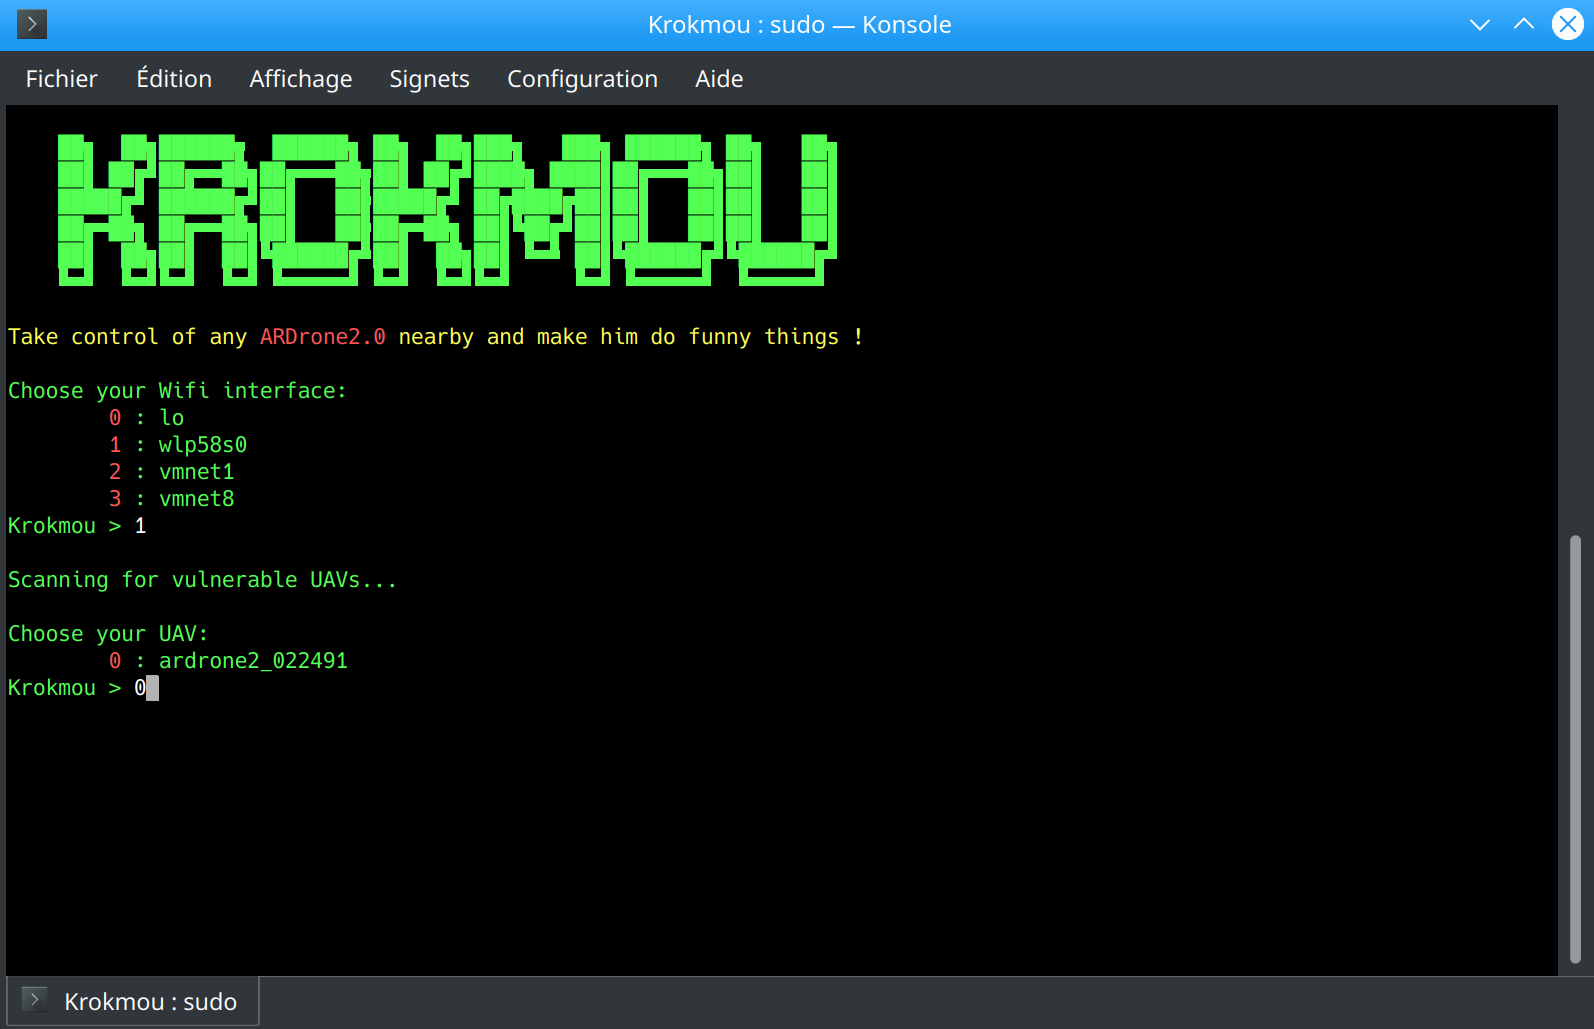
\includegraphics[scale=0.35]{images/opening.png}
  \caption{Initialisation de l'application}
\end{figure}

\subsection{Menu principal}
Le menu principal de l'application permet de sélectionner une des trois attaques afin de la réaliser sur le drone auquel l'attaquant s'est connecté précédemment.

\begin{figure}[H]
  \centering
  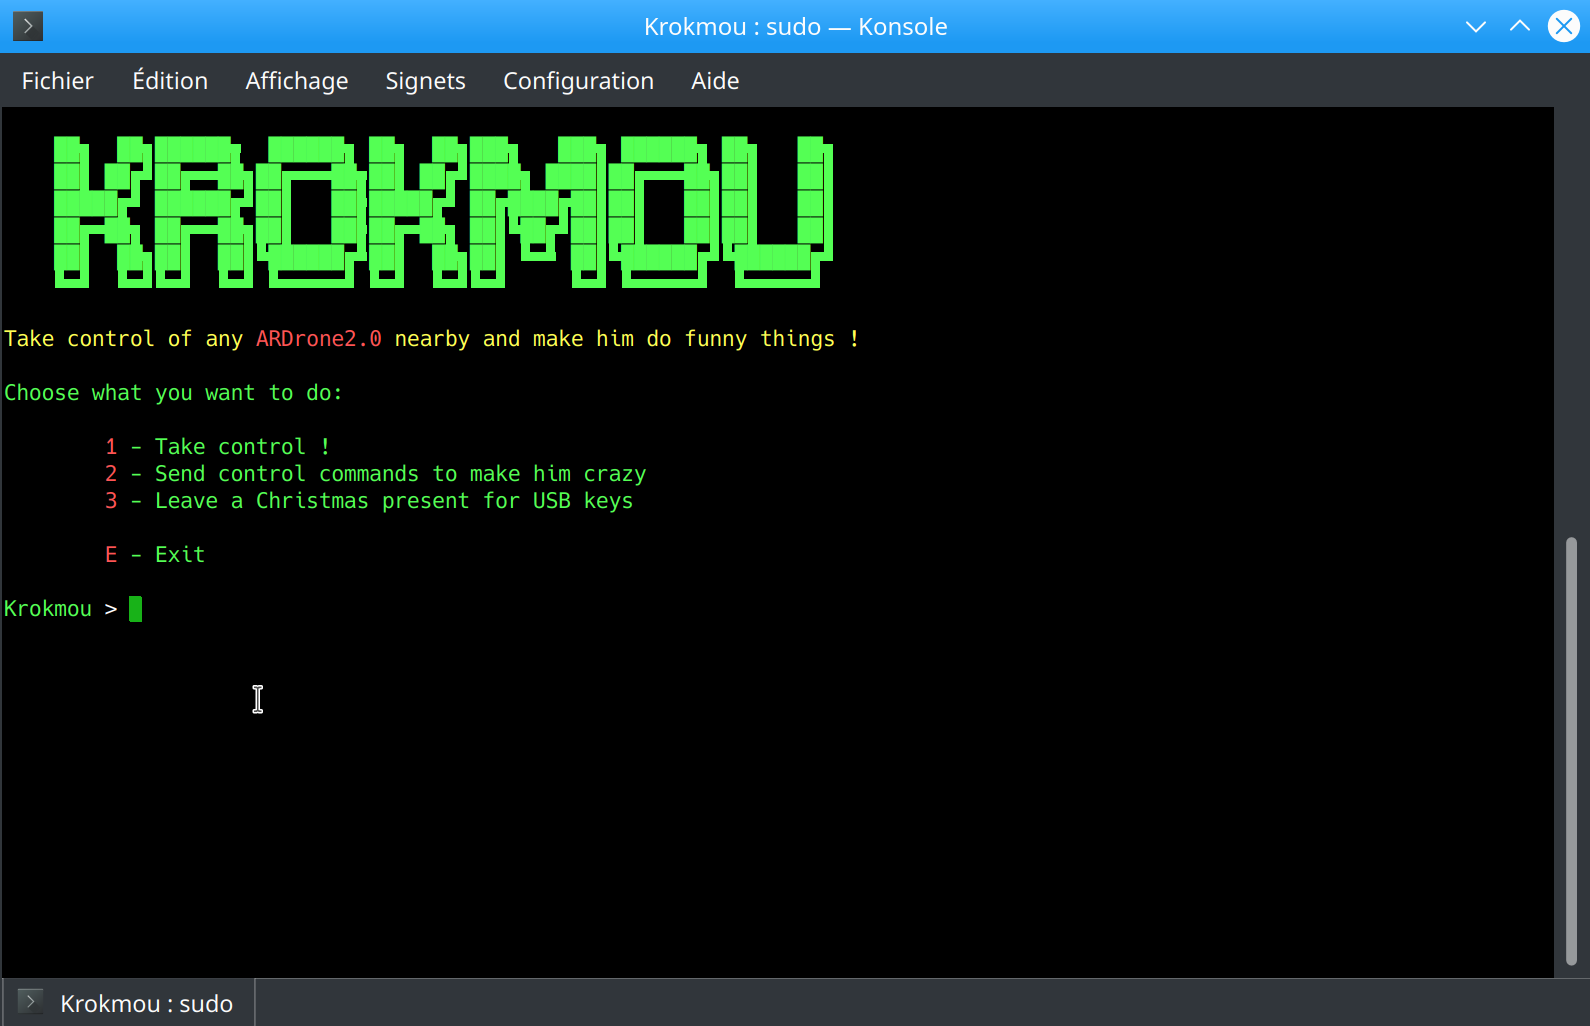
\includegraphics[scale=0.35]{images/main_menu.png}
  \caption{Menu principal de l'application}
\end{figure}

\subsection{Prise de contrôle du drone}
Cette option du menu permet à l'attaquant de prendre le contrôle du drone à la place de l'utilisateur légitime grâce à l'attaque décrite précédemment dans ce rapport. Le contrôle du drone se réalise au travers du navigateur Web et d'un serveur \textbf{Node.js} issu du dépôt Github suivant: (\url{https://github.com/functino/drone-browser}).

\begin{figure}[H]
  \centering
  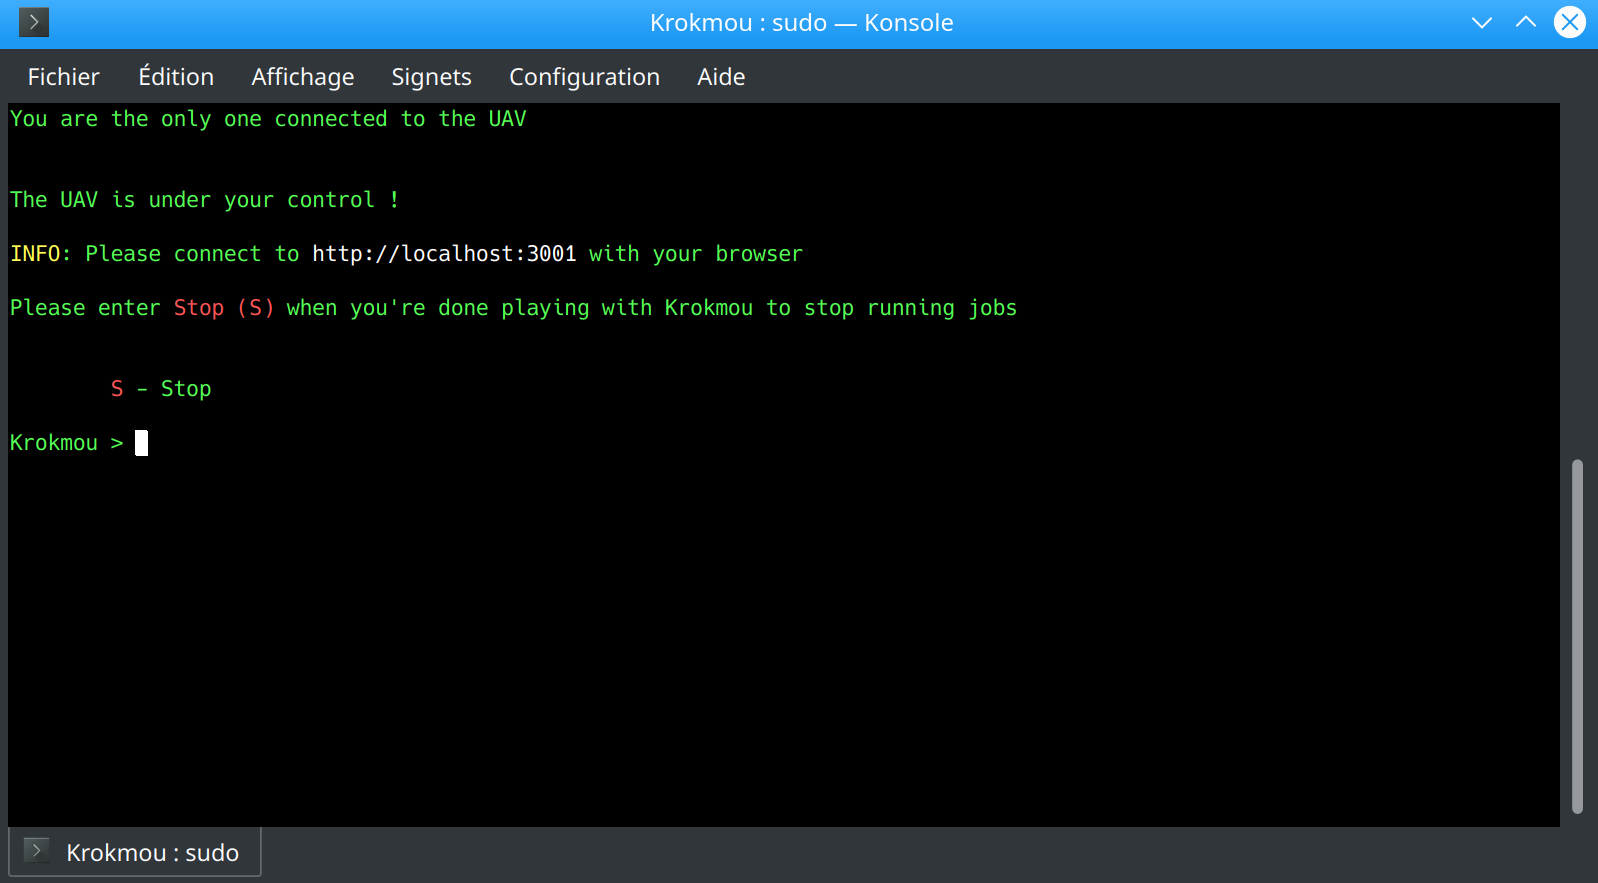
\includegraphics[scale=0.35]{images/taking_control.png}
  \caption{Prise de contrôle du drone par l'application}
\end{figure}

\begin{figure}[H]
  \centering
  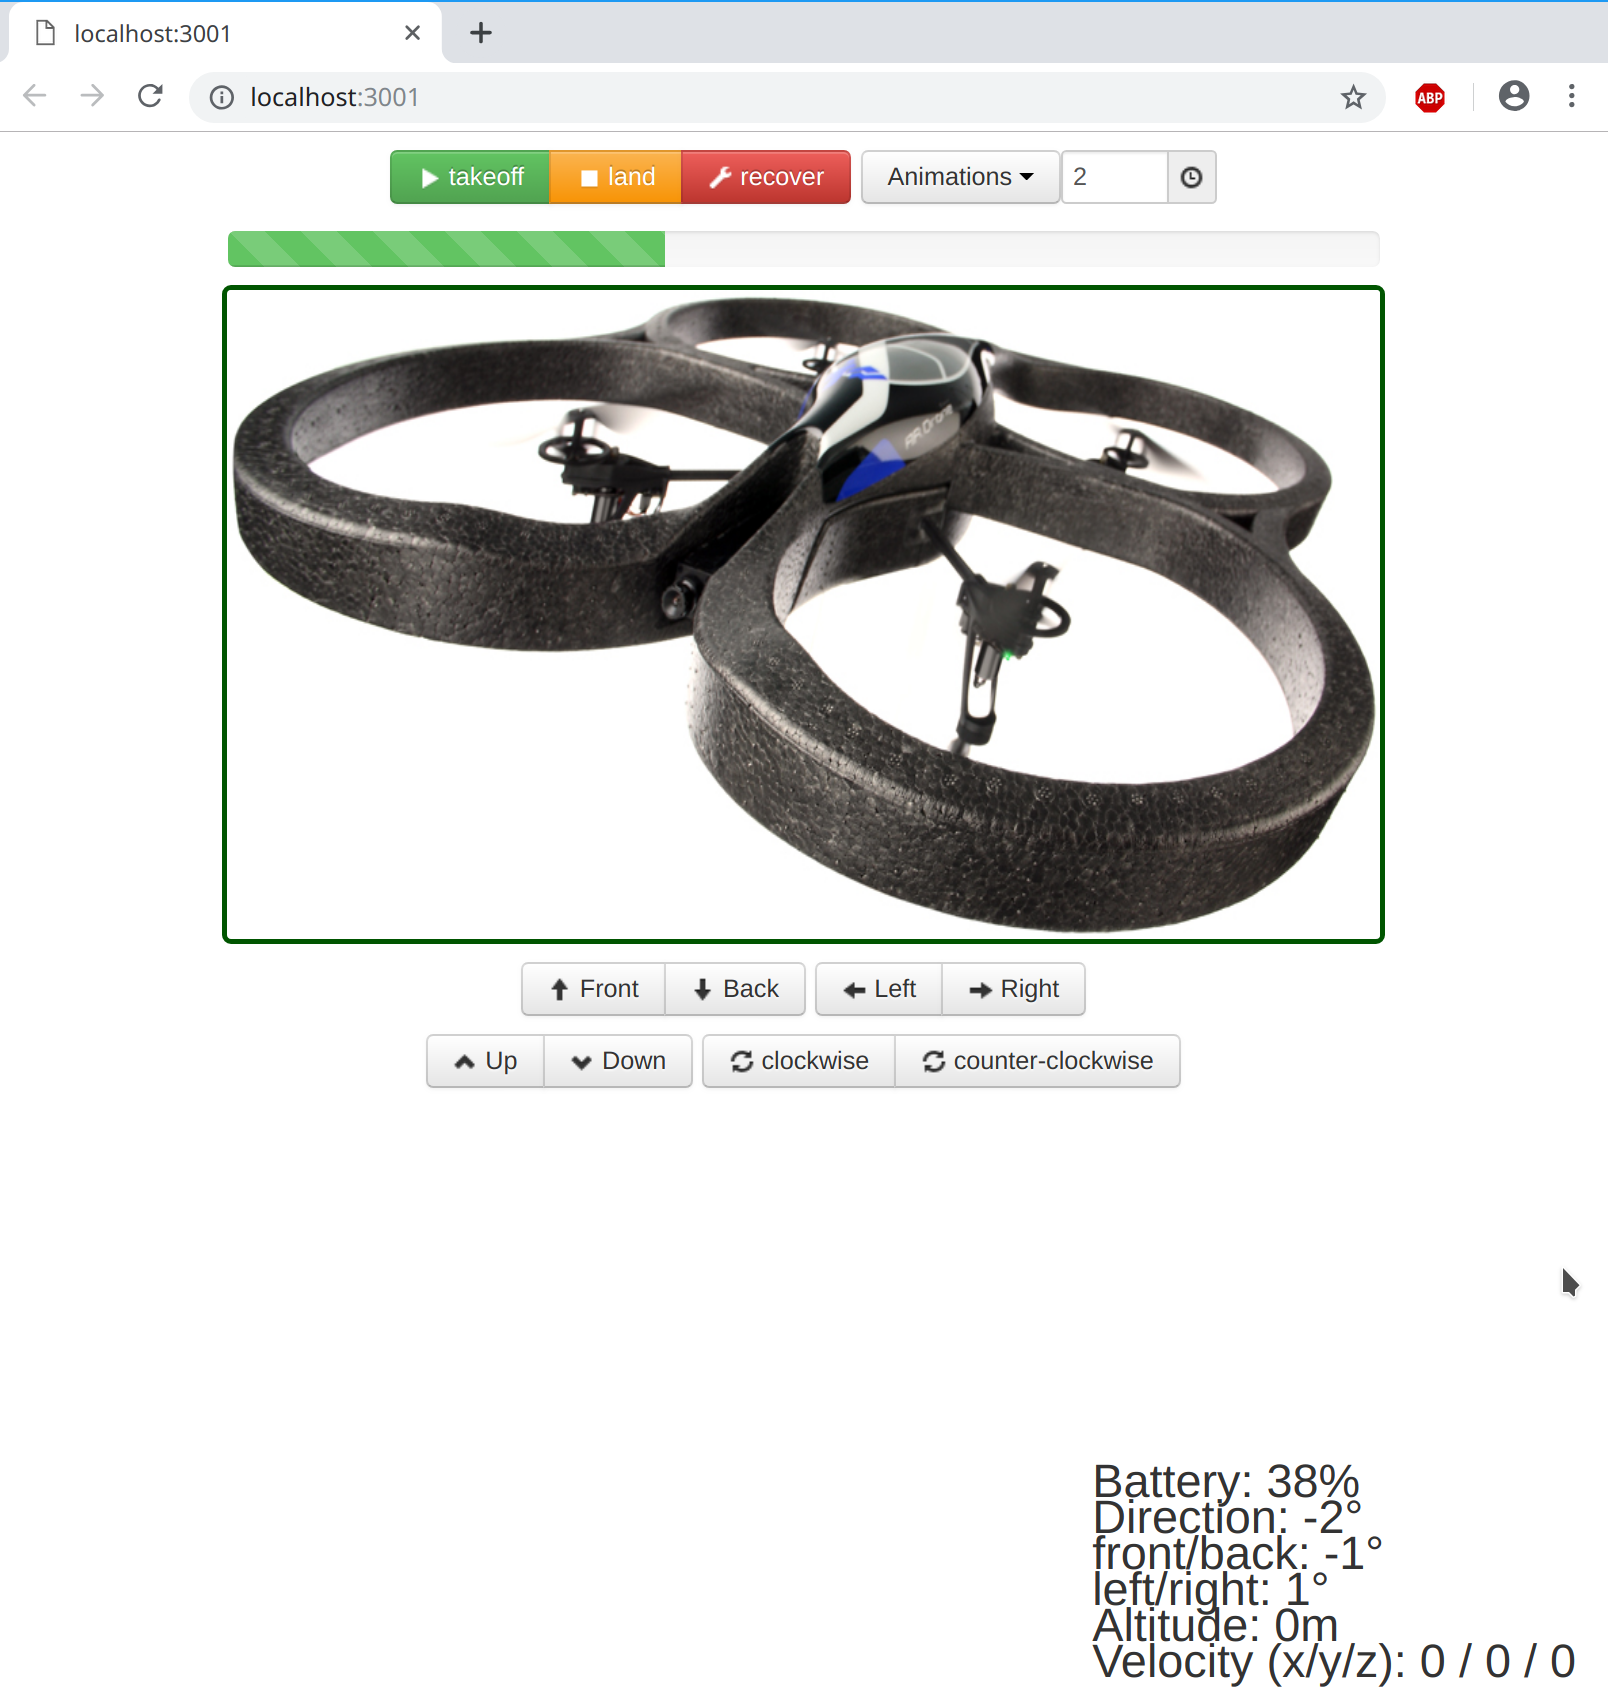
\includegraphics[scale=0.35]{images/control_application.png}
  \caption{Interface de contrôle web}
\end{figure}

\subsection{Injection de commandes}
Ce sous-menu permet à l'attaquant d'envoyer des commandes au drone en laissant le contrôle du drone au client légitime. Les différentes injections de commandes possibles sont présentées dans l'affichage du contrôleur pour l'injection de commandes.

\begin{figure}[H]
  \centering
  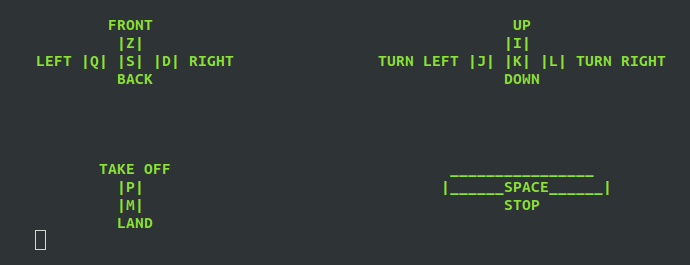
\includegraphics[scale=0.6]{images/injection_command_controler.png}
  \caption{Sous-menu d'injection de commandes}
\end{figure}

Il est donc possible de faire avancer/reculer, d'aller à gauche/droite, de monter/descendre, de tourner à gauche/droite selon l'axe vertical et de décoller/atterrir. L'utilisation du contrôleur se fait donc à l'aide du clavier. \\
Le client légitime garde le contrôle du drone à la seule condition que le drone soit dans le même état (en vol/au sol) que celui du client légitime avant l'injection de commandes.

\subsection{Dépose de virus sur le drone}
Cette option permet d'exploiter une vulnérabilité laissant à l'attaquant un contrôle total du drone. Dans le cadre de la démonstration, l'application dépose un virus et un fichier sélectionné par l'utilisateur sur le drone. Ce fichier sera copié sur toute clé USB qui sera connectée au drone. Celle-ci sera par conséquent considérée comme infectée. Par défaut, l'application dépose le virus et une image sur le drone. C'est cette image qui sera copiée sur toute clé USB connectée au drone toujours à des fins de démonstration. Cependant, l'attaquant peut indiquer le chemin d'un fichier de son choix au moment où l'application lui propose afin de remplacer cette image.

\begin{figure}[H]
  \centering
  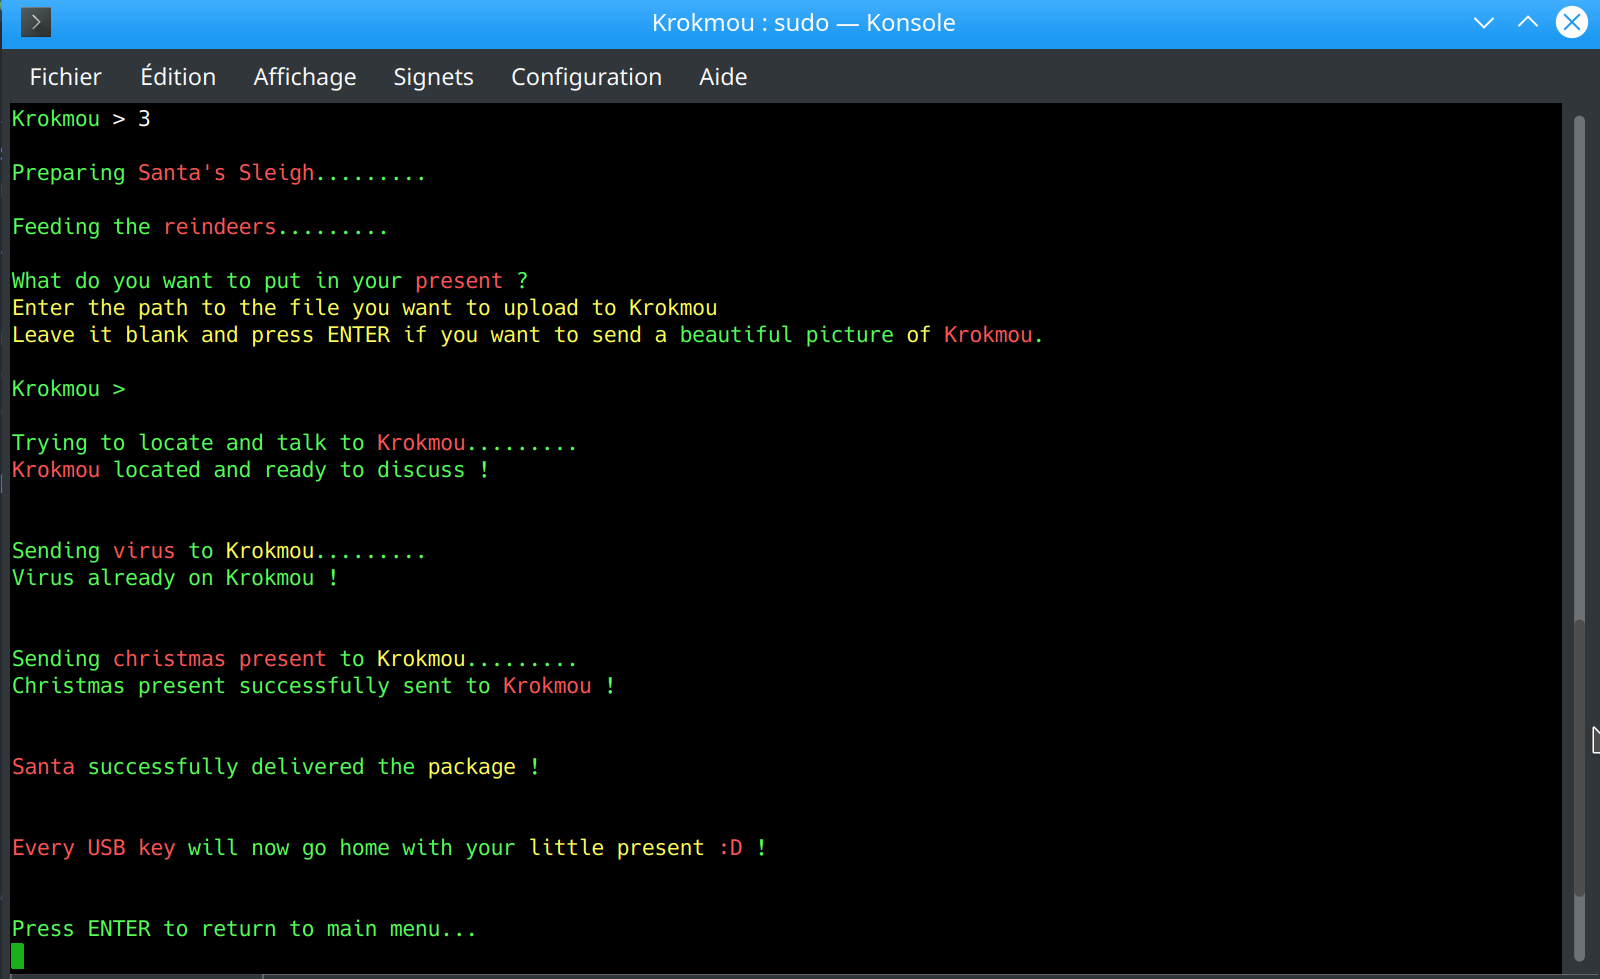
\includegraphics[scale=0.3]{images/virus.png}
  \caption{Envoi du virus et du fichier sur le drone}
\end{figure}


\section{Sécurisation du drone}
Comme nous avons pu le voir, cet ARDrone 2.0 de \textbf{Parrot} rencontre de nombreux problèmes de sécurité et reste vulnérable à certaines attaques. L'une des vulnérabilités principales se trouve dans le point d'accès Wifi qui est un réseau ouvert donc accessible à toute personne se trouvant à portée du drone.

\subsection{Sécurisation via le Wifi}
\paragraph{Modification du point d'accès}
L'une des premières mesures pour ce drone serait donc une modification de ce point d'accès Wifi en y ajoutant un mot de passe afin de le rendre privé. Afin de minimiser les risques de compromission du réseau, l'utilisation de la norme WPA2 semble optimale. Après un rapide état de l'art sur Internet, il semblerait que personne ne se soit réellement penché sur le problème mais un fichier bash présent sur le drone, \textit{wifi\_setup.sh}, laisse présager que cette modification est possible.

\paragraph{Utilisation du drone comme un client}
Une autre solution consisterait à utiliser le drone non comme un point d'accès mais comme un client du Wifi.
Afin de pouvoir connecter le drone à un réseau en WPA2, il est nécessaire d'effectuer de la compilation croisée sur le module \textit{wpa\_supplicant}, qui gère les connections au wifi WPA2 sur les environements Unix. En effet, le drone possède une architecture ARM et non x86. Heureusement, la communauté est riche de talent, et ce travail a déjà été fait dans ce dépot Github: \url{https://github.com/daraosn/ardrone-wpa2}.

Cette manipulation se fait en plusieurs étapes:
\begin{itemize}
  \item installation du module \textit{wpa\_supplicant} sur le drone.
  \item connecter le drone au point d'accès WPA2 du téléphone.
  \item faire en sorte que le drone ait l'adresse 192.168.1.1. Changer l'adresse du point d'accès pour le permettre.
  \item contrôler le drone via le téléphone.
\end{itemize}

Avec ce procédé, on bénéficie alors d'une connexion sécurisée avec le drone que l'on pilote. Attention toutefois à bien choisir son mot de passe. En effet, si une personne arrive à se connecter au Wifi du téléphone, le drone redevient totalement vulnérable. La contrainte de cette technique est donc l'utilisation d'un point d'accès Wifi annexe avec la bonne adresse IP pour le routeur. Dans un premier temps, nous l'avons essayer rapidement avec un iPhone comme point d'accès mais celui-ci n'offre pas un réseau interne du type \textit{191.168.1.0/24} et il n'est pas possible de modifier cela dans les paramètres.

\subsection{Renforcement du numéro de séquence}
Il a été mis en évidence que le drone interprète toutes les commandes avec un numéro de séquence supérieur au sien. Même s'il est nettement supérieur à celui en cours, il sera interprété.\\
Une idée de renforcement de ce dernier est de prévoir le numéro de séquence probable. On sait que le client envoie des paquets UDP de façon régulière. On peut donc mettre en place une fourchette pour estimer le numéro de séquence suivant. Ainsi le numéro de séquence doit toujours être supérieur à celui en cours mais aussi inférieur à celui probable en connaissant la fréquence d’envoi du client légitime. On pourra également ajouter une petite marge d'erreur sur la borne supérieur mais il faut que cette dernière soit raisonnable.\\\\
Avec ce procédé, on bénéficie alors d'une connexion sécurisée avec le drone que l'on pilote.

\subsection{Connexion à distance}
Comme vu précédemment, le drone dispose de 3 services \textbf{TCP} ouverts dont le service \textbf{FTP} et le service \textbf{Telnet}. Ces deux services sont très utiles pour la dépose de fichiers ou encore la maintenance du drone à distance. Mais ils représentent surtout deux portes ouvertes sur le drone et sont donc de réelles menaces pour la sécurité du drone.

\begin{figure}[H]
  \centering
  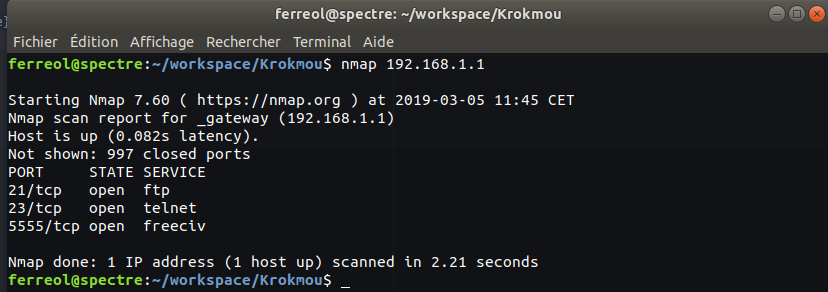
\includegraphics[scale=0.5]{images/scan_drone}
  \caption{Services disponibles sur le drone}
\end{figure}

La solution la plus simple serait de supprimer ces deux services et de les remplacer par un seul et même service, le service \textbf{SSH}. En effet, celui-ci combine l'aspect transfert de fichier de \textbf{FTP} et l'accès à distance de \textbf{Telnet} en plus d'offrir des garanties de sécurité avec notamment la présence d'un authentification à la connexion. Attention cependant, cette solution n'est viable que si le mot de passe par défault est changé à la première utilisation du drone.


\section{Conclusion}
L'ARDrone 2.0 de \textbf{Parrot} est donc un drone grand public de loisirs qui présente des vulnérabilités importantes. La principale est le réseau Wifi ouvert qui autorise toute personne à portée de signal Wifi à se connecter au drone. La sécurisation du réseau Wifi créé par le drone en utilisant un réseau Wifi WPA2 permettrait de combler cette faille majeure. Dans un second temps, les ports ouverts sur le drone donnent accès à des services sur celui-ci sans authentification de la part de l'utilisateur. Ainsi un accès \textbf{FTP} permettant un accès aux fichiers du drone est laissé à tout utilisateur connecté au réseau Wifi de celui-ci. De plus, faille plus importante, un service \textbf{Telnet} est également accessible fournissant un accès \textbf{root} sur le drone à tout utilisateur connecté au Wifi. Cet accès est une faille majeure car elle permet à un attaquant d'avoir tous les droits sur le drone et ainsi de pouvoir faire ce qu'il veut au niveau du système d'exploitation de celui-ci. Dans un troisième temps, le contrôle du drone présente également des failles dans la gestion des commandes envoyées par l'utilisateur. En effet, il est possible pour un attaquant de forger de fausses commandes en se faisant passer pour l'utilisateur légitime et ainsi de contrôler le drone. Le drone n'effectue pas d'authentification des commandes qu'il reçoit et ne vérifie donc pas que celle-ci viennent de l'utilisateur légitime. Pour terminer, nous avons démontrer qu'il était possible d'exploiter ces différentes failles afin de prendre le contrôle du drone mais elles peuvent également servir à réaliser des attaques de type Déni de Service sur celui-ci et ainsi bloquer la connexion entre lui et le client.
\newline La place de plus en plus importante que prennent ces drones de loisir dans l'espace aérien va nécessiter dans le futur que ceux-ci ne présentent plus ce type de failles majeures afin d'empêcher que des attaquants puissent en prendre le contrôle ou  plus simplement puissent réfuter le contrôle de l'aéronef à son utilisateur légitime, et ceci pour des raisons de sécurité vis à vis des autres aéronefs évoluant dans le même espace.








\end{document}
